\documentclass[runningheads]{llncs}
\usepackage[utf8]{inputenc}
\usepackage{mathtools}
\usepackage{algorithm}
\usepackage{algorithmic}

\usepackage{graphicx}
\usepackage{caption}
\usepackage{subcaption}
\usepackage{siunitx}
\usepackage[linguistics]{forest} % Trees

%\usepackage{algpseudocode}
%\usepackage{algorithmicx}
\usepackage{amssymb}

\usepackage{hyperref} % For clickable \href{} URLs


% Colored table cells
%\usepackage[table,xcdraw]{xcolor}

\title{A Critical Analysis of the\\Boolean Satisfiability Problem}
\author{Simeon Wuthier}
%
\authorrunning{S. Wuthier}

\institute{
    \textit{Department of Computer Science}\\
    \textit{University of Colorado, Colorado Springs}\\
    \email{swuthier@uccs.edu}\\
}

\date{15 December, 2020}


\begin{document}
\maketitle
\footnotetext[0]{The format of this paper is in ACM; Lecture Notes in Computer Science (LLNCS)}

\section{Introduction}

The Boolean satisfiability problem (SAT) is a propositional logic problem with applications spanning across physics, mathematics, computer science, cryptography, artificial intelligence, and many others. As a widely used modeling framework for solving combinatorial problems, SAT is the first NP-complete decision problem, introduced in 1971 from the Cook-Levin theorem \cite{cook1971complexity}. The theorem states that the SAT problem is NP-complete, and that any other NP problem can be reduced to SAT in polynomial time by using a deterministic Turing machine. Because SAT is NP-complete, unless \emph{$P = NP$}, all algorithms that solve SAT instances require a worst-case time complexity that is exponential. Despite this potential restriction on the algorithm's performance, modern SAT algorithms have become very effective at tackling instances that require a large search space, allowing significant improvements that would otherwise make some problems unrealistic for the traditional brute-force approach. Since the structure of the problem has been taken advantage of, with a handful of mechanisms that achieve a much faster execution time \cite{silva2003grasp}\cite{moskewicz2001chaff}\cite{een2003extensible}\cite{goldberg2007berkmin}, the SAT problem has never achieved an execution time that is polynomial in the worst-case. If such an algorithm was to exist, theoretically or not, then the Cook-Levin theorem would allow every NP problem to reduce to it, making other challenging problems such as the knapsack problem, hamiltonian path problem, traveling salesman problem, as well as protein folding and countless other problems optimally solvable in polynomial time. Likewise, if such a problem were to be proven impossible to achieve polynomial time, then \emph{$P \neq NP$}, making it clear that some problems simply cannot ever be solves quickly.  %Being one of the most studies problems in theoretical computer science

\subsection{Contributions}
This study tackles the SAT problem head-on, in order to build a powerful working implementation, and discuss the current optimizations at play, as well as the optimizations made by the worlds fastest algorithm, and the corresponding algorithm analysis for each. The original implementation made from this project\footnote{Working implementation can be found at \url{https://simewu.github.io/SAT-solver}} was build in JavaScript and is cross-platform.

\section{Preliminaries}
The SAT problem can be described as follows.

\begin{definition}
Let $x_1,...,x_m$ be Boolean variables that are part of a formula, $F$, where $x_i\in\{true, false\} \forall x\in F$. A \textbf{literal} can be either $x$ or $\neg x$ (logical not). A \textbf{clause} is some number of literals joined by $\lor$ (logical or) and surrounded by parenthesis. The Boolean \textbf{formula}, $F$ joins some number of clauses with $\land$ (logical and). Then given F with Boolean variables X=\{$x_1,...,x_m$\}, decide whether or not there exists a function $f\to\{true, false\}$ such that when one replaces $x_i$ by $f(x_i)$ in S, the evaluated Boolean sentence will be logically true, where $f(S)=true$. We say that $S$ is \textbf{satisfiable}. $F$ is in \textbf{conjunctive normal form}\footnote{A conjunction is another word for \emph{and}, while a disjunction is means a \emph{or}.}, which states that all clauses must only be joined by a logical and, and all literals must only be joined by a logical or.
\label{def:SAT}
\end{definition}

While the conjunctive normal form may appear to apply to a very restricted subset of Boolean propositions, Whitesitt proves that every Boolean proposition can be reduced to conjunctive normal form \cite{whitesitt2012boolean}.

\subsection{Universal Formatting}
\label{sec:dimacs}
The DIMACS format is a universal conjunctive normal form syntax guideline that allows all SAT applications to be understandable to all SAT solvers \cite{challenge1993satisfiability}. The file format ends with the \emph{.cnf} file extension and they all contain a header. Comments begin with the letter \emph{c}, and data is delimited by one or more spaces. The first non-comment must be \emph{p cnf} followed by the number of \emph{variables} used in the SAT instance, then the number of clauses (or rows of data) in the file.


\section{Performance Strategies}
While the traditional brute force method of iterating through the permutation of all variable possibilities is sufficient for smaller programs, the time complexity is in $\Omega(2^n)$ making it unreasonable for larger SAT instances.

\begin{figure*}[h]
\begin{forest}
  [
    [\textit{$x_1=0$}
        [\textit{$x_2=0$}
            [\textit{$x_3=0$}
            ]
            [\textit{$x_3=1$}
            ]
        ]
        [\textit{$x_2=1$}
            [\textit{$x_3=0$}
            ]
            [\textit{$x_3=1$}
            ]
        ]
    ]
    [\textit{$x_1=1$}
        [\textit{$x_2=0$}
            [\textit{$x_3=0$}
            ]
            [\textit{$x_3=1$}
            ]
        ]
        [\textit{$x_2=1$}
            [\textit{$x_3=0$}
            ]
            [\textit{$x_3=1$}
            ]
        ]
    ]
  ]
\end{forest}
\caption{The brute-force decision tree to solve a SAT problem with three variables. A brute force solver must traverse each node, where the leaf nodes will have an assignment for every variable and can be plugged in to check for satisfiability. After visiting every leaf node, a brute-force solver will be able to conclude unsatisfiability by means of proof by exhaustion.}
\end{figure*}

The implementation presented in this paper uses a few core optimizations, which are as follows: unit propagation, two-watched literals, no-good learning, and conflict-directed back-jumping, which are discussed in further detail in Section~\ref{sec:experimentation}.

\subsection{World Record}
As of 2020, the current world record belongs to Hansen \emph{et al.} \cite{hansen2019faster} at a time complexity of $O(1.307^n)$, which uses a method known as biased PPSZ. Fourteen years earlier, Paturi \emph{et al.} introduced the PPSZ algorithm \cite{paturi2005improved} which has a time complexity of $O(1.308^n)$. Both algorithms assume a unique $3-SAT$ instance, which requires exactly three variables within each clause, and has a single unique solution, making it non-ambiguous. The optimization included adding a heuristic to the literal selection, as opposed to the traditional PPSZ. The pseudocode for biased PPSZ can be found in Algorithm~\ref{alg:biased-ppsz}. This time complexity was derived from the time complexity $2^{S_kn-\delta|\mathcal{D}|}$, where $S_k$ is the upper probability that a variable is guessed by the PPSZ algorithm, not requiring additional bias. $n$ is the size of the input, and $\delta$ refers to the gain over the PPSZ algorithm for the average of $x,y,z$, which is the three variables within each clause of a $3-SAT$ instance. $\mathcal{D}$ is the maximal set of disjoint clauses assuming that the clauses of $\mathcal{D}$ are unnegated, where $|\mathcal{D}|$ is the number of clauses \cite{hansen2019faster}. After assigning the worst-case variable values to the time complexity, the formula gave a time complexity of $O(1.306995^n)$. They mention that many improvements and optimizations can be made on their work, to decrease this value further. 

\begin{algorithm}[h]
\caption{The biased-PPSZ algorithm, with a time complexity of $O(1.307^n).$}
\label{alg:biased-ppsz}
\begin{algorithmic}[1]
    \STATE // $\beta$ is an assignment variable
    \STATE // $\pi$ is a permutation of the variables, ordered strategically
    \STATE // $F$ is the input k-CNF formula, and $P$ is the heuristic
    \STATE \textbf{function} \textsc{BiasedPPSZ}($\beta, \pi, F, P$)
    \STATE $V \xleftarrow{}$ var($F$), the variables of $F$
    \STATE $\alpha \xleftarrow{}$ the empty assignment on $V$
    \FOR{$x\in V$ in the order of $\pi$}
        \IF{$P(F,z)\in\{0,1\}$}
            \STATE $\alpha(x)\xleftarrow{}P(F,x)$
        \ELSE
            \STATE $\alpha(x)\xleftarrow{}\beta(x)$
        \ENDIF
        \STATE $F\xleftarrow{}F|_{x=\alpha(x)}$
    \ENDFOR
    \IF{$F$ has been satisfied}
        \RETURN $\alpha$
    \ELSE
        \RETURN \texttt{failure}
    \ENDIF
 \end{algorithmic}
\end{algorithm}

\section{Experimentation}
\label{sec:experimentation}
%unit propagation, two-watch literals, no-good learning, and conflict-directed back-jumping, which are discussed in further detail in Section~\ref{sec:experimentation}.

As stated in the previous section, the implementation of this paper uses unit propagation, two-watched literals, no-good learning, and conflict-directed back-jumping. This section will describe each of these mechanisms, then discuss the environment, design choices, and how validation was achieved.

\subsection{Unit Propagation}
A \emph{unit clause} is defined as a clause with a single literal in it that has not been set (i.e. the only literal with an unknown value). Because all clauses are joined by a logical and, every clause must evaluate to $true$, when only a single unset literal is present if it takes the form of $\neg x_i$, $x_i=false$, otherwise $x_i=true$. \emph{Unit propagation} is the practice of discovering a unit clause and setting the value, which may trigger other clauses to become unit clauses. Following this chain of events allows the additional assignment of variables with a certainty of their value.

\subsection{Two-watched Literals}
Two-watched literals is a technique that speeds up unit propagation detection. Because unit propagation is only triggered when a clause has one remaining variable to be set, instead of iterating through each variable within a clause to check for unit propagation, two-watched literals allow a great reduction in the number of computations required to determine if unit propagation is possible. The technique consists of only monitoring two unset literals within each clause. When one of these variables becomes set, there is the possibility for a unit propagation. To be certain, the algorithm will look for another unset literal. If no unset literal is found, then the other watched variable will receive a value by way of unit propagation, otherwise, the algorithm will begin watching the newly found unset variable. This allows performance optimization when the size of each clause is greater than two.

\subsection{No-good Learning}
\emph{Nogood} learning is a technique used alongside backtracking, where failures are analyzed through the decision tree, and \emph{nogoods} are derived from the variable assignments, to avoid reaching the same failure in future runs \cite{nogoodlearningdefinition}. Lecoutre \emph{et al.} apply this into the constraint satisfaction problem in order to demonstrate the effectiveness of such a mechanism. The study found that no-goods work more efficiently when a restart policy is used, by almost one order of magnitude \cite{lecoutre2007nogood}.

\subsection{Conflict-directed Back-jumping}
The implementation of this paper uses a restart policy known as conflict-directed back-jumping, which is triggered after \emph{nogood} learning when a conflict is found. Proposed in 1994, conflict-directed back-jumping is based on checking whether each constraint caused an inconsistency, and if so the mechanism will jump further, and avoid the extra computational overhead \cite{prosser1994binary}. 

\begin{figure*}[h]
\centering
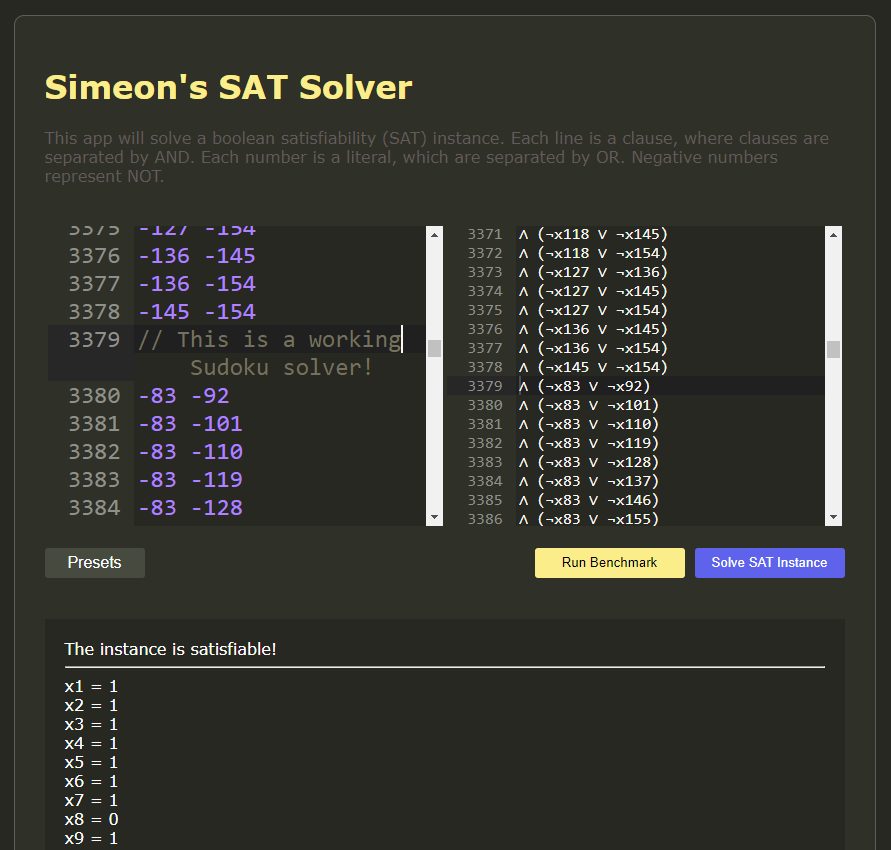
\includegraphics[width=0.8\textwidth]{Figures/screenshot.png}
\caption{The SAT solving implementation presented in this project, working on solving a Sudoku. It is hosted at \url{https://simewu.github.io/SAT-solver} and the original source code at \url{https://github.com/simewu/SAT-solver}. The left box is the editor, the right box shows the instance mathematical format, which updates in real-time, and the lower box provides the results consisting of either the solution to the SAT instance (satisfiable or unsatisfiable) along with the variable's that prove the solution or the results from the benchmark. Both functionalities can be triggered by clicking the blue button, or the yellow button, respectively.}
\label{fig:screenshot}
\end{figure*}

\subsection{Environment and Design Choices}
The application underwent numerous design choices that favor usability over performance. The choice to use JavaScript in a web application was the biggest of the design choices, as it allowed creating an interactive application at the cost of CPU resources. Likewise, the application cannot be comparable to traditional SAT solvers, since JavaScript is slower than C, and interpreted rather than compiled. Design choices also include an interactive user interface, as opposed to a terminal-style application. Figure~\ref{fig:screenshot} shows the interface along with a description of the controls. For added usability, the interface was split into two halves, each running the Ace library\footnote{The Ace code editor is available at \url{https://ace.c9.io}} which allows high-performance code editing. Both editors display the same information, however, the left editor is in DIMACS format, while the right displays the SAT instance in mathematical terms.

Regarding design choices of the algorithm itself, the \texttt{solveSAT} function takes in an array of clauses, where each clause is an array of literals, and each literal is an integer either negative or positive depicting whether or not it is negated or not, respectively. A \texttt{State} class is used to capture the current state of the solver, by holding information about its recursive depth, the assignment of the variables and clauses, including the newly learned clauses. Cloning the state at any given point will save the entire SAT solving instance, allowing for greater modularity and future functionality, such as pausing the solver and resuming at a different time, or spreading out the CPU utilization across time in order to not overwhelm the system. The \texttt{Variable} class, similar to the \texttt{State} class, is responsible for holding the state of every variable, such as whether or not it is set, the sign, and two-watched array, which the solver looks at to check for unit propagation.

Because the algorithm initially chooses the variable assignments randomly, the SAT solver finds solutions randomly, and any ambiguities can be discovered by repeatedly solving the instance, otherwise, it can be concluded with the increasing probability that the SAT instance is unique. Section~\ref{sec:validating-correctness} elaborates on this by providing a unique instance along with one that is ambiguous.

The entire application is maintained within a single \emph{index.html} document, consisting of everything except the Ace editor library, which is held in the \emph{libs} folder. The source code \footnote{The solver is available at \url{https://github.com/simewu/SAT-solver}} is stored within Github, to allow for version control and additional features, such as hosting, and collaboration in the future.

\subsection{Validating Correctness}
\label{sec:validating-correctness}
Because SAT is such a famous problem in theoretical computer science, there exist many DIMACS files (explained in Section~\ref{sec:dimacs}) that are SAT instances aimed at solving specific problems, or benchmarking how effective the solver is. The following example provides a unique solution ($x_1=true, x_2=false, x_3=true$), that a SAT solver can use to verify correctness.
$$(\neg x_1 \lor x_3)\land (x_1 \lor x_2)\land \neg x_2$$
Ambiguities can be introduced by adding literals or clauses that provide multiple correct variable assignments. The following instance contains exactly two solutions, $\{x_1=true, x_2=false\}$ and $\{x_1=false, x_2=true\}$:
$$(x_1 \lor x_2)\land (\neg x_1 \lor \neg x_2)$$

More complex instances can be tested, such as the one provided by Kwon \emph{et al.} that solves Sudokes \cite{kwon2006optimized}, which was incorporated into the application under $\textsc{Presets}\xrightarrow{}\textsc{Functioning Sudoku}$. The results have been compared with a famous solver known as \emph{MiniSAT} \cite{sorensson2010minisat}, showing that the solver is capable of more complex instances without conflict.

\section{Empirical Analysis}
A benchmarking button was included in the application. This feature generates an instance with $C$ clauses consisting of $L$ random literals ($x_i$ or $\neg x_i$). The performance of concluding that it is either SAT or UNSAT is logged. $C$ and $L$ are varied. The first experiment made $C$ the control ($C=512$) and $L$ the independent variable ($C\in {1, 2, 4, 8, 16, 32, 64, 128, 512, 1024, 2048, 4096, 8192}$) in Figure~\ref{fig:literal_perf}, and $L$ the control with $C$ being the independent variable in Figure~\ref{fig:clause_perf}, and the time duration in milliseconds (ms) was the dependent variable. This experiment found a solver bias in favor of $C$ as opposed to $L$, showing that the number of clauses is more efficient to scale.

\begin{figure*}[h]
\begin{subfigure}{0.5\columnwidth}
    \centering
    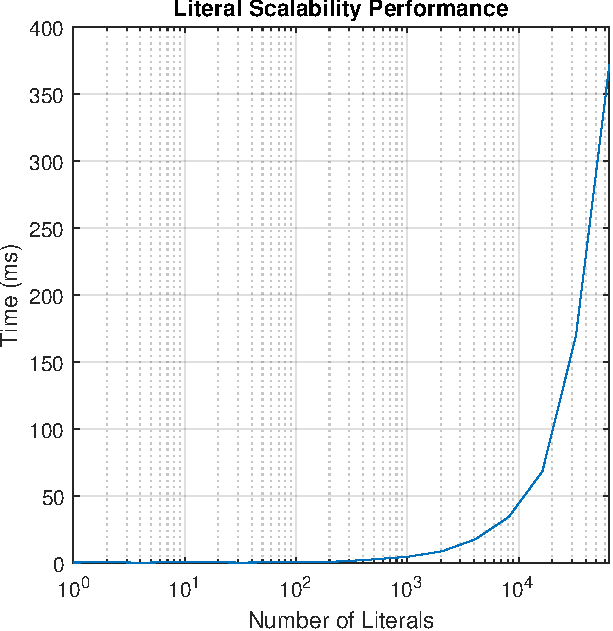
\includegraphics[width=1\textwidth]{Figures/literal_perf.pdf}%\hfill
    \caption{Time duration of number of literals. The control was the number of clauses, at 512 clauses.}
    \label{fig:literal_perf}
\end{subfigure}
\hfill
\begin{subfigure}{0.5\columnwidth}
    \centering
    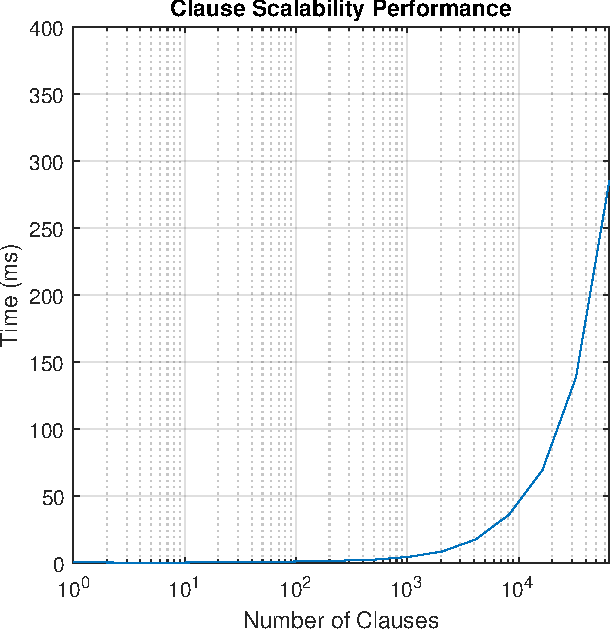
\includegraphics[width=1\textwidth]{Figures/clause_perf.pdf}%\hfill
    \caption{Time duration of number of clauses. The control was the number of literals, at 512 clauses.}
    \label{fig:clause_perf}
\end{subfigure}
\end{figure*}

The next experiment did not consist of any control variables, but instead  made both $C$ and $L$ independent variables in a nested \emph{for} loop, where $C, L \in {1, 2, 4, 8, 16, 32, 64, 128, 256, 512, 1024, 2048, 4096, 8192}$. As shown in Figure~\ref{fig:clause_literal}, the trade-off between $L$ and $C$ scale almost proportionally.

\begin{figure*}[h]
    \centering
    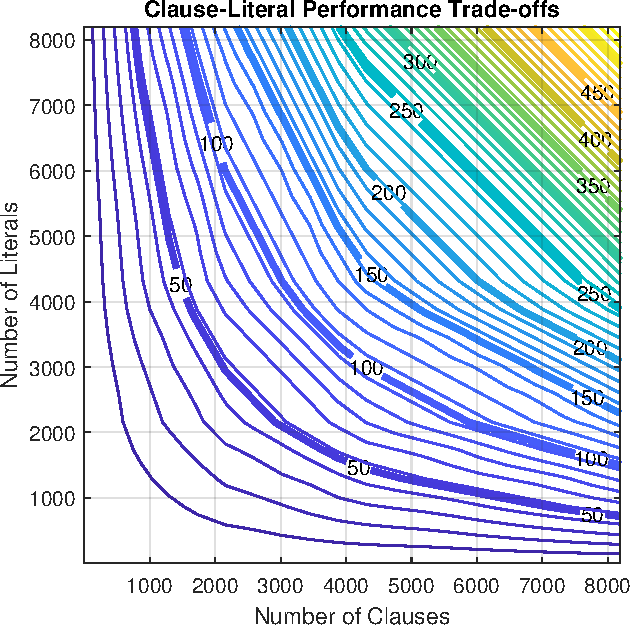
\includegraphics[width=0.7\textwidth]{Figures/clause_literal.pdf}
    \caption{Three-dimensional contour of number of clauses to number of literals, where the color represents the total execution time of the SAT instance. Ten samples were taken per data point, and the average was plotted.}
    \label{fig:clause_literal}
\end{figure*}


\begin{figure*}[h]
    \centering
    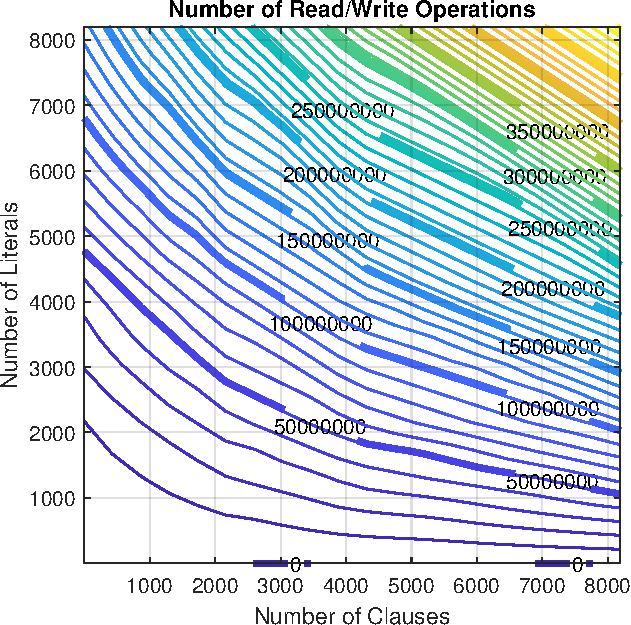
\includegraphics[width=0.7\textwidth]{Figures/num_operations.pdf}
    \caption{Three-dimensional contour of number of clauses to number of literals, where the color represents the total number of read/write operations for each instance. Ten samples were taken per data point, and the average was plotted.}
    \label{fig:num_operations}
\end{figure*}

\begin{table}[]
\centering
\tiny
\begin{tabular}{l|l}
Input Size & Operations \\ \hline
1          & 3          \\
2          & 19.4       \\
4          & 98.8       \\
8          & 478.4      \\
16         & 1835.2     \\
32         & 7702.4     \\
64         & 31910.4    \\
128        & 125376     \\
256        & 494873.6   \\
512        & 1935974    \\
1024       & 7941018    \\
2048       & 31660646   \\
4096       & $1.26\times 10^8$   \\
8192       & $5.02\times 10^8$  
\end{tabular}
\caption{Assuming $C=L$ (i.e. the number of clauses is equal to the number of literals), the number of operations increases at an exponential rate.}
\label{tab:operations-table}
\end{table}

\subsection{Read/Write Operations}
The next experiment was done by counting the number of variable reads, and the number of variable writes required to solve the SAT instance. Figure~\ref{fig:num_operations} visualizes the results and shows how increasing the number of clauses significantly increases the number of operations when compared to increasing the number of literals. To have a more complete analysis, assuming $C=L$, the number of operations increases exponentially, as seen in Table~\ref{tab:operations-table}, where an input size of 8192 has $5.02\times 10^8$.


\clearpage

\subsection{Additional Information}

Of all the randomly generated SAT instances, where the number of clauses and number of literals varied between 1 and 8192, this study found that \textbf{86.53\%} of the instances were satisfiable, leaving only 13.47\% as unsatisfiable. The instance generator was unbiased, where $P(x_i=true) = 0.5$, and 19,600 total instances were generated, showing that this is a somewhat universal behavior.

\noindent\rule{12.5cm}{0.4pt}
\\

The application can be accessed at \url{https://simewu.github.io/SAT-solver}.
\footnotesize
\bibliographystyle{splncs04}
\bibliography{references.bib}
\end{document}

